\documentclass[11pt]{article}
\usepackage[utf8]{inputenc}
\usepackage[sfdefault]{roboto}		
\usepackage[T1]{fontenc}
\usepackage[spanish,es-tabla]{babel}
\usepackage{graphicx}
\usepackage[hidelinks]{hyperref}
\usepackage[a4paper]{geometry}
\usepackage{listings}
\geometry{top=3cm, bottom=3cm, left=3cm, right=3cm}
\hypersetup{
	colorlinks=true,
	linkcolor=blue,
	filecolor=magenta,
	urlcolor=cyan,
}

\graphicspath{ {images/} }

\title{KVM (\textit{Linux Kernel Virtual Machine})}
\author{Antonio Jos\'e Lara Peña
		\\ Manuel Horacio Cañero Torres
		\\ Hugo Teruel Muñoz
		\\ Mar\'ia Rodrigo González
		\\ Daniel Monjas Miguélez}


\begin{document}
\maketitle
\newpage
\tableofcontents
\newpage
\section{Introducción}
El presente documento tiene por objeto principal hablar detalladamente sobre KVM, una máquina de virtualización creada por la empresa israelí Qumranet. \\

La motivación principal de este trabajo es la de poder profundizar más en la materia de Sistemas Operativos, permitiéndonos abstraer conocimientos de distintas fuentes, para así tener que contrastar información e interiorizar el temario de la asignatura. \\

La Virtualización es el tema elegido para este trabajo. Para desarrollar este tema, se propone investigar sobre una forma de virtualización entre las que se encuentra Linux Containers, Linux Kernel Virtual Machine (KVM) y Linux User Mode Linux (UML). Entre estas tres opciones, nos hemos decantado por la segunda. \\

La elección del tema responde a dos circunstancias: la primera de ellas el desconocimiento que teníamos sobre esta forma de virtualización ya que hemos trabajado con otras como el User Mode Linux en clase de prácticas de la asignatura
pero no hemos tenido la ocasión de utilizar esta; la segunda es porque nos parecía llamativo que estuviera la palabra kernel en el nombre ya que es mencionado con frecuencia en los contenidos de la materia y pensamos en que podríamos aprender más sobre ella realizando esta investigación. \\

La información está distribuida en distintos apartados, los cuales unidos dan una imagen bastante clara sobre KVM. Entre los apartados del proyecto nos podemos encontrar con qué es KVM y cómo se describe dentro del mundo de la virtualización, una descripción de la instalación, el funcionamiento y las principales aplicaciones de esta forma de virtualización. \\

La temática del proyecto ayuda a la experimentación, ya que con solo tener un ordenador podemos ver de forma práctica lo que es KVM, lo cual siempre facilita a la comprensión del objeto de estudio. \\

En definitiva, este trabajo nos sirve para aumentar nuestros conocimientos en el mundo de los sistemas operativos y sobre todo en el mundo de las formas de virtualización, lo cual es indispensable para poder avanzar en nuestra camino como futuros ingenieros informáticos.

\section{¿Qué es KVM?¿Cómo se describe dentro del mundo de la virtualización?}
\subsection{¿Qué es KVM}
KVM (\textit{Kernel-based Virtual Machine}) es una tecnología de virtualización completa de código abierto para procesadores x86 y x86\_64 que dispongan de soporte para virtualización (Intel VT or AMD-V), siendo actualmente el hipervisor de virtualización oficial del kernel de Linux. Usando KVM, uno puede ejecutar múltiples máquinas virtuales que ejecutan imágenes sin modificar de Linux o de Windows. Relacionandolo con el temario visto en clase KVM sería \textit{HW-assisted virtualization}.\\

Está formada por un módulo del núcleo denominado \textit{kvm.ko}, que proporciona la infraestructura de virtualización central y un módulo específico del procesador, \textit{kvm-intel.ko} o \textit{kvm-amd.ko}. \\
\\

Se creó en 2006 por la empresa \textit{Qumranet} como parte de un proyecto centrado en una solución VDI(\textit{Virtual desktop infraestructure}) para clientes Windows y se integró a la versión del kernel principal de Linux en el año posterior, más concretamente en la versión 2.6.20 de este sistema operativo. Así es posible aprovechar cada nueva función de Linux sin requerir ninguna ingeniería adicional. Este hecho no implica que haya soporte comercial ni que se incluyan las herramientas necesarias. \\

Puesto que KVM es una tecnología de virtualización de código abierto varias empresas han apostado por ella dedicandose a la mejora de la misma, entre las que se encuentran:

\begin{itemize}
\item IBM ha sido una empresa ha apostado fuerte por KVM, teniendo numerosos desarrolladores trabajando sobre esta máquina virtual en distintas áreas como la gestión de memoria y mejorando el rendimiento y el subsistema de E/S virtual. 
\item Red Hat, esta empresa utiliza KVM como unico hipervisor para todos sus productos de vritualización, y continuamente mejora el código del kernel con las distribuciones de la la comunidad KVM( \textit{véase \href{https://www.linux-kvm.org/page/Main_Page}{Comunidad KVM}}).
\end{itemize}


Básicamente, KVM es un módulo cargable del Kernel que permite al SO Linux actuar como un hipervisor bare metal tipo 1, que puede verse como un software centrado en la ejecución de máquinas virtuales. Por ser de tipo 1 también tiene que tratar otras tareas mas predeterminadas como por ejemplo drivers de dispositivos, gestión de memoria o planificación de procesos.


\subsection{¿Cómo se describe dentro del mundo de la virtualización?}
La virtualización es una tecnología que permite ejecutar varios sistemas operativos simultáneamente en una misma máquina. En un entorno virtualizado, cada sistema operativo tiene la ilusión de residir en una máquina propia(\textit{véase \ref{Funcionamiento} }, disponible eternamente para él.  Para conseguir esto es necesario un programa (denominado virtualizador o hipervisor, según la técnica concreta que se utilice) que se encargue de arbitrar el uso del hardware. Para ello intercepta las operaciones privilegiadas y simula sus efectos sobre un dispositivo virtual, también simulado. \\

\begin{figure}
\centering
\caption{Esquema de funcionamiento de la virtualización}
\label{Funcionamiento}
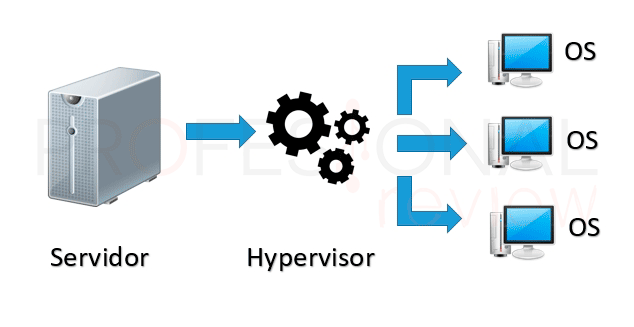
\includegraphics[width=1\textwidth, scale=1]{virtualizacion-tuto02.png}
\end{figure}

Dentro del mundo de la virtualización distinguimos dos tipos que definimos para aclarar la diferencia entre ello y que en futuras menciones se tenga claro su función:

\begin{itemize}
\item \textbf{Hipervisores tipo 1 o \textit{bare metal}}: Los hipervisores de este tipo se ejecutan sobre el hardware al mismo nivel que se ejecutaría el sistema operativo. Como ejemplos de hipervisores de tipo 1 tenemos KVM, Xen y VMware.(Peralta, 2012)
\item \textbf{Hipervisores de tipo 2 o \textbf{hosted}}: Los hipervisores de tipo \textit{hosted} se ejecutan, a diferencia de los anteriores, sobre un sistema operativo que a su vez ejecuta sobre el mismo hardware físico. Como ejemplo de hipervisores de este tipo tenemos Qemu y Wine.(Peralta, 2012)
\end{itemize}

\subsubsection{¿Qué relación tiene con QEMU?}
KVM se suele utilizar muy comunmente en conjunto con QEMU por lo que vamos a dar una breve descripción de su relación.

QEMU es un emulador de procesadores basado en la traducción dinámica de binarios, es decir, realiza la conversión del código binario de la arquitectura fuente o host, en código entendible por la arquitectura huésped o la VM. El resultado de usar QEMU es poder ejecutar el código original como si se estuviera ejecutando en la máquina emulada. Por ejemplo, se podría ejecutar código escrito para el procesador ARM en su máquina basada en Intel. \\

QEMU y KVM trabajan juntos. Los desarrolladores de KVM aprovecharon la arquitectura QEMU y básicamente crearon un nuevo modelo de CPU en QEMU. Este nuevo tipo de modelo tiene una lógica específica de KVM. Así las llamadas al sistema que se harían de forma nativa pasan por del módulo KVM para que la ejecución se ejecute de forma nativa en la CPU -- mientras que QEMU se utiliza para proporcionar el resto funcionalidad (emular los dispositivos). \\

Además, cuando las personas se refieren al hipervisor KVM, en realidad se refieren a la combinación QEMU-KVM. KVM necesita QEMU (u otro emulador) para la funcionalidad completa como hipervisor. QEMU es autosuficiente y KVM es realmente un módulo del kernel de Linux para la explotación de extensiones VT que actúa como controlador de las capaciones de CPU físicas. Así puedes notar entonces que QEMU necesita a KVM poder aumentar su rendimiento. Por otro lado KVM por sí solo no puede proporcionar la solución de virtualización completa. \\

En general, la importancia de KVM va más allá de su uso como virtualizador: ha sido la primera tecnología de virtualización que ha pasado a formar parte del núcleo Linux. Las razones por las que eso ocurrió fue su limpia implementación, que no requiere la inclusión de un hipervisor y por lo tanto es una solución puramente Linux. En la Figura \ref{interfaz qemu} podemos observar la interfaz de QEMU. En ella se aprecia las opciones de iniciar un Sistema operativo desde disco duro, reparar un sistema instalado, etc. No debemos olvidar que los sistemas ejecutados desde QEMU no se ejecutan directamente sobre el hardware, sino que son un proceso que dispone de recursos que KVM le asigna y que hace llamadas al sistema y ejecuta código kernel por medio de KVM.

\begin{figure}
\centering
\caption{Interfaz gráfica de QEMU}
\label{interfaz qemu}
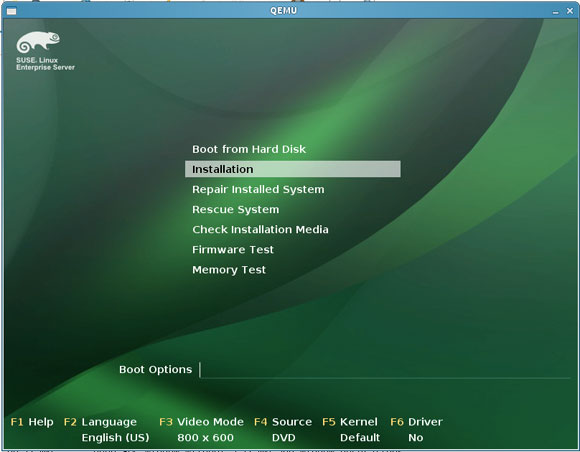
\includegraphics[width=1\textwidth, scale=1]{qemu.jpg}
\end{figure}

\section[Principales características, ventajas e inconvenientes]{Principales características, ventajas e inconvenientes que presenta dentro del mundo de la virtualización}
\subsection{Principales caracterísitcas}
\subsubsection{Seguridad}
KVM utiliza una combinación de \textit{security-enhanced Linux (SELinux)} y virtualización segura (\textit{sVirt}) para la seguridad y el aislamiento mejorados de máquina virtual. \textit{SELinux} establece los límites de seguridad para las máquinas virtuales. \textit{sVirt} amplía las capacidades de SELinux, lo que permite que la seguridad de control de acceso obligatorio (MAC) se aplique a las máquinas virtuales huéspedes y evita los errores manuales de etiquetado.

\subsubsection{Almacenamiento}
KVM puede usar cualquier almacenamiento compatible con Linux, incluidos algunos discos locales y el almacenamiento conectado a la red (NAS: \textit{Network Attacherd Storage}). La entrada/salida de rutas múltiples mejora el almacenamiento y proporciona redundancia. KVM también es compatible con sistemas de archivos compartidos de tal manera que las imágenes de las máquinas virtuales se puedan compartir entre varios hosts. Las imágenes de disco dan soporte al aprovisionamiento ligero para asignar almacenamiento a pedido en lugar de desde el inicio.

\subsubsection{Compatibilidad con el hardware}
KVM puede usar una amplia variedad de plataformas de hardware certificado y compatibles con Linux. Como los proveedores de hardware contribuyen de forma periódica al desarrollo del kernel, las funciones de hardware más recientes a menudo se adoptan rápidamente en el kernel de Linux.

\subsubsection{Gestión de memoria}
KVM hereda las funciones de gestión de memoria de Linux, incluidos el acceso a la memoria no uniforme y la fusión de la misma página del kernel. La memoria de una máquina virtual se puede intercambiar, tiene el soporte de grandes volúmenes para un mejor rendimiento, y se puede compartir o respaldar por un archivo de disco.

\subsubsection{Migración en vivo} \label{migración en vivo}
KVM permite la migración en vivo, esto es la capacidad de mover una máquina virtual en funcionamiento de un host físico a otro sin que se interrumpa el servicio. La máquina virtual permanece encendida, las conexiones de red permanecen activas y las aplicaciones continúan ejecutándose mientras se reubica la máquina virtual. KVM también guarda el estado actual de la máquina virtual para que se pueda almacenar y retomar posteriormente.

\subsubsection{Rendimiento y escalabilidad}
KVM hereda el rendimiento de Linux, ya que puede escalar hasta satisfacer la carga requerida si la cantidad de máquinas huéspedes y las demandas crece. KVM permite que las cargas de trabajo de las aplicaciones más exigentes se virtualicen, y es la base para muchas configuraciones de virtualización empresarial, como los centros de datos y las nubes privadas (mediante OpenStack).

\subsubsection{Latencia más baja y mayor prioritización}
El kernel de Linux cuenta con extensiones en tiempo real que permiten que las aplicaciones basadas en máquinas virtuales se ejecuten con una latencia más baja y una mejor priorización (frente a sin sistema operativo). El kernel también divide los procesos que requieren largos períodos de computación en componentes más pequeños, que luego se programan y se procesan en consecuencia.

\subsection{Ventajas e inconvenientes que presenta dentro del mundo de la virtualización}
Ventajas:
\begin{itemize}
\item Está diseñado para procesadores x86, centrando en una virtualización total.
\item No se modifica el kernel de GNU/Linux.
\item Solamente es un módulo del núcleo que no necesita parches.
\item Contiene soporte de paravirtualización.
\item KVM funciona en todo tipo de máquinas, servidores, ordenadores de escritorio o portátiles.
\item Migración en vivo de máquinas virtuales(\textit{véase}\ref{migración en vivo}).
\item Tiene administración via web, gráfica y consola.
\item La administración de las máquinas virtuales se hae por medio de un usuario mortal.
\item Podemos utilizar el comando kill para matar auinas virutales ya que con KVM son reconocidos como procesos.
\item Permite ejecutar múltiples máquinas virtuales cada una con su propia instancia.
\item KVM proporciona un entorno para programas que es identico al de la máquina original.(Popek, G. J., Goldberg, R. P. 1974. Formal requirements for virtualizable third-generation architectures. Communications of the ACM 17(7): 412-421)
\end{itemize}

Desventajes:
\begin{itemize}
\item Se necesita disponer de un procesador con soporte para virutalización hardware, como son los procesadores con tecnología AMD-V e Intel-VT
\item No tiene ni el soporte ni el apoyo económico y tecnológico que tienen otras plataforma de virtualización
\item No tiene una interfaz gráfica que se bonita y sencilla de usara para configurarlo y administrarlo.
\item No dispone de herramientas sofisticadas para la gestión de servidores y para las gestión/creación de máquinas virtuales.
\end{itemize}


\section{Descripción de la instalación y funcionamiento}
\subsection{Descripción de la instalación}
Teniendo en cuenta que KVM está integrado en kernel de Linux, se requiere soporte para virtualización. Por lo que para asegurarnos de tener un dispositivo compatible, ejecutaremos la siguiente orden:
	\begin{lstlisting}[frame=single]
		$ cat /proc/cpuinfo | grep vmx #para CPUs Intel
		$ cat /proc/cpuinfo | grep svm #para CPUs AMD
	\end{lstlisting}

\begin{figure}
\centering
\caption{Asistente para la creación de máquinas virtuales}
\label{Asistente}
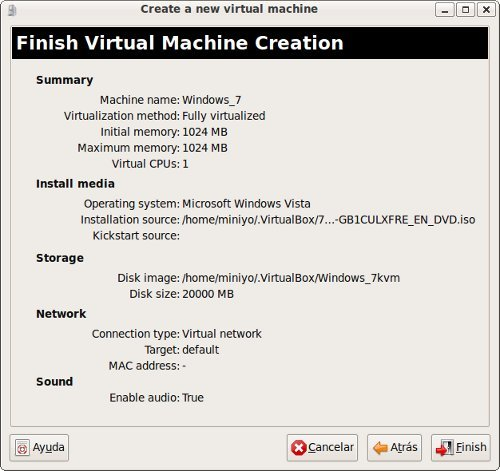
\includegraphics[width=0.8\textwidth, scale=1]{ejemplo.jpg}
\end{figure}
	
En caso de que dicha orden no devuelva nada, significa que no se dispone de un dispositivo compatible con KVM.Si la ejecución de la orden devuelve lo que se busca, confirmaremos la compatibilidad y la instalación se realiza con las órdenes (para Linux
10.4 o superior):

	\begin{lstlisting}[frame=single]
	$ sudo apt-get install qemu-kvm libvirt-bin 
	ubuntu-vm-builder bridge-utils
	$ sudo adduser $USER kvm
	\end{lstlisting}
	
En primer comando instalará:
\begin{enumerate}
\item \textit{libvirt-bin} proporciona \textit{libvirtd}, que se necesita para administrar KVM y QEMU. 
\item \textit{qemu-kvm}
\item \textit{ubuntu-vm-builder}, un comando muy potente que sirve para la construcción de máquinas virtuales.
\item \textit{bridge-utils}, sirve de puente desde la red a las máquinas virtuales.
\end{enumerate}

Una vez realizado, y tras haber reiniciado sesión, si todo ha salido bien, el dispositivo ya está listo para comenzar a instalar máquinas virtuales, para lo que aparecerá una nueva pestaña en \textit{Herramientas del Sistema}(\textit{véase} \ref{Asistente}).



\subsection{Funcionamiento}
KVM convierte Linux en un hipervisor de tipo 1 (sin SO), es decir, está integrado en el kernel. Todo hipervisor precisa de componentes al nivel del sistema operativo, como administrador de memoria, planificador de procesos, pila de entrada o salida, etc. para ejecutar máquinas virtuales, KVM cuenta con todos los componentes descritos puesto que es parte del proceso kernel de Linux. Las máquinas virtuales se implementan como un proceso regular de Linux, programada por el planificador estándar de Linux con Hardware virtual dedicado como tarjeta de red, adaptador de gráficos, CPU, memoria y discos.

\section{Aplicaciones}
KVM es una opción para la virtualización de código abierto integrada en Linux. Está incluida en este desde la versión 2.6.20. \\

Permite que las cargas de trabajo se virtualicen, siendo la base para muchas configuraciones de virtualización empresarial, como los centros de datos y las nubes privadas (mediante OpenStack) \\

KVM es importante para la ejecución de máquinas virtuales utilizando imágenes de disco que contienen sistemas operativos sin modificar. Cada máquina virtual tiene su propio hardware virtualizado: tarjeta de red, discos duros, tarjeta gráfica\ldots \\

Es importante el uso de KVM en una distribución Linux como la de Red Hat Enterprise Linux, pues se amplían las capacidades de KVM, permitiendo el intercambio de recursos entre guests, compartir bibliotecas comunes, optimizar el rendimiento del sistema\ldots \\

Otra aplicación es la migración a una plataforma de virtualización basada en KVM, que nos permite tener la capacidad para inspeccionar, modificar y mejorar el código fuente detrás de su hipervisor. Se lleva a cabo sin acuerdo de licencia empresarial, pues no hay que proteger ningún código fuente (es suyo). \\

Una de las principales aplicaciones de KVM es OpenStack Compute(Nova) (se trata de un módulo de OpenStack) que es un controlador de estructura cloud computing. KVM es una de las opciones disponibles para la tecnologiía de hipervisor de este módulo de OpenStack.



\section{Conclusiones}
Hemos aprendido que KVM es una tecnología de virtualización completa de código abierto que requiere que el procesador tenga soporte para virtualización. \\

También hemos aprendido que KVM se trata de un módulo integrado en el kernel lo que permite que los sistemas operativos ejecutados en las máquinas virtuales facilitadas por KVM sean practicamente igual de eficientes que un sistema operativo ejecutado directamente sobre la máquina física, pues KVM proporciona los recursos hardware de forma directa, pues se trata de virtualización asistida por hardware, luego las peticiones de recursos no hace falta realizarlas al sistema operativo y que este los planifique posteriormente, sino que KVM realiza directamente la asignación sin necesidad de intermediarios.\\

Además hemos aprendido que KVM requiere de algún VMM(\textit{Virtual Machime Manager}) que trabaja conjuntamente con KVM de forma que las máquinas que el VMM emula ejecutan directamente su código en el \textit{host} por medio de KVM. \\

También hemos aprendido que KVM es una tecnología de virtualización que se utiliza especialmente en el cloud computing y hemos visto un poco más a fondo su papel en OpenStack, donde KVM funciona como hipervisor en el módulo Compute(Nova) de OpenStack. \\

También hemos visto como se puede instalar KVM y un el funcionamiento del mismo, destacando que antes de instalar KVM se debe comprobar que la máquina en la que se quiere instalar disponga de las extensiones para soporte de virtualización necesarias. \\

Hemos aprendido también que KVM tiene varias características interesantes, entre las cuales destacaremos la migración en vivo, que nos ha resultado especialmente interesante. 


\newpage
\begin{thebibliography}{x}
	\bibitem{RED} \textit{Tecnología de virtualización(KVM), Red Hat \url{https://www.redhat.com/es/topics/virtualization/what-is-KVM}}
	\bibitem{KVM} \textit{Comunidad KVM \url{http://www.linux-kvm.org/page/Main_Page}}
	\bibitem{GEN} \textit{Virtualización con KVM, virtualización de código abierto, Genbeta \url{https://www.genbeta.com/a-fondo/virtualizacion-con-kvm-virtualizacion-de-codigo-abierto}}
	\bibitem{DEB} \textit{KVM installation, Ubuntu Documentation \url{https://help.ubuntu.com/community/KVM/Installation}}
	\bibitem{VIRT} \textit{Virtualización de sistemas operativos, Gradiant \url{https://www.gradiant.org/noticia/virtualizacion-de-sistemas-operativos-2/}}
	\bibitem{RDLAB} \textit{Virtualización de servidores del RDlab, Xavier Peralta Ramos \url{https://www.cs.upc.edu/~gabriel/files/PFC-XavierPeralta.pdf}}
	\bibitem{galvarado} \textit{Virtualización a fondo,¿Cuales son las diferencias entre KVM y QEMU?¿Son sinónimos?, Guillermo Alvarado \url{https://galvarado.com.mx/post/kvmqemu/}}
	\bibitem{admin} \textit{KVM, Administración de sistemas operativos \url{http://www.adminso.es/index.php/KVM}}
	\bibitem{Pop} \textit{Popek, G. J., Goldberg, R. P. 1974. Formal requirements for virtualizable third-generation architectures. Communications of the ACM 17(7): 412-421}
\end{thebibliography}

















\end{document}